% Subsystem report for Datapath control system, typeset for the LaTeX processor.
% Copy the next line and put your initials instead of JL.
\fancyfoot[R]{JL}
\section[Datapath Control]{Acquisition Unit Datapath Control}
% Description of function or purpose
\subsection{Description}
For the data acquisition hardware, a flexible base was needed to manage the 
flow of data from the analog or digital input modules to the host PC. It was 
also desired to allow the host PC to manage the configuration of the input 
modules themselves. The datapath control subsystem regulates the flow of data 
from the input modules\index{input modules} and serializes it for output to 
the host PC software. It provides a multiplexed bus for analog and/or 
digital interface modules and also provides a control interface for those 
modules. The bus width was set at 10 bits, which was the minimum size for
 accepting output from the analog input module designed for use with this 
datapath.

Figure \ref{fig:datapath diagram} shows a block diagram of the datapath system. The complete schematic is located at in the appendix at page \pageref{sch:datapath}. 
The Serial Control Unit (SCU)\index{SCU}, when enabled, accepts data over the bus from 
either the digital input module or the analog input module. The bus control 
itself is managed by the Master Control Unit (MCU)\index{MCU}. The MCU also 
manages the optional control lines for the input modules and supports up to 
6-bit widths for input module configuration. The MCU also manages the on/off 
and reset functionality of the SCU itself. The commands are represented with 8-bit opcodes that are forwarded over the serial link through the SCU to the MCU. 

\begin{figure}[hbp]
\caption{Datapath block diagram}
\begin{center}
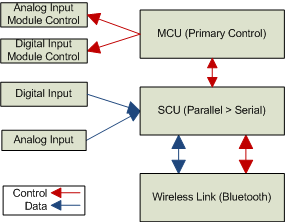
\includegraphics[width=4in]{../drawings/datapath_block.png}
\end{center}
\label{fig:datapath diagram}
\end{figure}
\subsection[Tradeoffs]{Design Decisions and Tradeoffs} 
Table \ref{tab:control comparison} lists an overview of the options considered
 for the datapath control subsystem. Cost refers to the per-unit cost of a 
given solution, Complexity is the amount of up-front design work that would
 need to be done to achieve basic functionality. TTL Logic and FPGAs are, for
 these considerations, similar. Both require much work to achieve some basic
 functionality but had very few limits in the the types of solutions that
 could be realized. FPGAs have an additional advantage over basic logic gates
 in that they are able to be relatively easily reconfigured or updating, which
 would make prototyping simpler. However, both solutions low-level
 implementations were considered to be too time-inefficient for this design.
 A general purpose "bare" microprocessor was also considered, but was quickly
 dismissed for similar reasons as FPGAs - the infrastructure required to get
 a general microprocessor functioning was also considered time-inefficient.

\begin{table}[bp]
\caption[Controllers]{Comparison of different control methods\cite{web:virtex4-cost}}
\begin{tabular}{l| c c c c c c}
		\multirow{2}{*}{\small{Control Type}} & \multirow{2}{*}{\small{Cost}} 
		& \multirow{2}{*}{\small{Complexity}} & \multirow{2}{*}{\small{Flexibility}} 
		& \multirow{2}{*}{\small{Speed}} 
		& \small{Time}\\
		&&&&&\small{Required}\\ \hline
		\small{Basic logic}  &     &      &      &     & \\
		  \small{gate chips} & \small{Low} & \small{High} & \small{High} & \small{Low} & \small{V. High} \\ 
		\small{FPGA} & \small{Average} & \small{High} & \small{High} & \small{Average} & \small{High}  \\
		\small{Microprocessor} &\small{ Average} & \small{High} & \small{Average} & \small{Average}
		 & \small{Average} \\
		\small{Microcontroller} & \small{Low} & \small{Low} & \small{Average} & \small{Average} & \small{Low} \\
\end{tabular}
\label{tab:control comparison}
\end{table}

Microcontrollers, however, are ideal for this type of application: they provide
 a flexible base and generally come packaged with different interfacing 
subsystems of their own for a low cost. In addition, many microcontrollers 
have a C compiler ported for their architecture, as well as the ability to
 reprogram them in-system. Table \ref{tab:MCU capabilities} outlines some of
 the capabilties of two microcontrollers that had been under consideration.
 While the the two devices are very similar, the Atmel MCU was chosen for its
 more flexible layout, multiple integrated interfaces, and the availability
 of a mature port of the GNU C Compiler for the device (and its family). The 
PIC required the use of the vendor-supplied compiler and IDE.
\begin{table}[bp]
\caption[Atmel and PIC MCUs]{Comparison of Atmel ATMega8515\cite{ds:ATMEGA8515
} and PIC18F1220\cite{ds:pic18f1220}\cite{web:pic18f1220}}
\begin{tabular}{l| c c c c c c}
\setlength{\tabcolsep}{1pt}
	       &      & \small{Pin}  & \small{Maximum} & \small{Ease}   &            &         \\
	\small{Device} & \small{Cost} & \small{Count} & \small{Speed}  & \small{of Use} 
	& \small{Interfaces} & \small{Features}\\\hline
	\multirow{3}{*}{\small{ATMega8515}} & \multirow{3}{*}{\small{Low}} & \multirow{3}{*}{\small{40}}
	& \multirow{3}{*}{\small{20Mhz}} & \small{High} 
	& \small{SPI,} & \small{Timers}\\
	           &     &    &       &      &\small{USART} & \small{External}\\
	& & & & & &\small{Memory}\\\hline
	\small{PIC18F1220} & \small{Low} & \small{18} & \small{40Mhz} & \small{Average} & 
	\small{USART} & \small{Timers} \\
	           &     &    &       &      &  & \small{10-bit ADC}\\
\end{tabular}
\label{tab:MCU capabilities}
\end{table}

The bus interface features two input ports and one output port. To effectively
 switch between the two inputs, those connections must be tri-stated. Thus, three 
74-series tri-state buffers were considered: the 74*244, the 74*245, and the 
74*621. Table \ref{tab:buffer comparison} outlines the key differences with 
the components considered. Ultimately, a 74*245 chip was selected for its 
flexibility and that there was a supply already on-site. 74*621s were found 
to be difficult to source in low quantites for a prototype. 74*244s could be 
used as well with some minor changes in glue logic, as well as 74*621s.

\begin{table}[bhp]
\caption[Buffer Comparison]{Comparison of different tri-state buffers}
\small
\begin{center}
\begin{tabular}{l| c c c c}
\setlength{\tabcolsep}{1pt}
	Device & Width & Bi-Directional & Cost & Availability \\\hline
	74*244 & 8     & No             & Low  & High\\
	74*245 & 8     & Yes            & Low  & High\\
	74*621 & 8     & Yes            & Low  & Low
\end{tabular}
\end{center}
\label{tab:buffer comparison}
\end{table}

Because the datapath control must serialize outgoing data, the performance
of the overall system contains a bottleneck at the point of the 
parallel-to-serial shift. Therefore, a secondary MCU is dedicated to
the operation of the parallel-to-serial operation, leaving actual datapath 
control to the primary MCU. This secondary MCU is another Atmel ATMega8515. A
different model of MCU would suffice, but using a second ATMega8515 allows  
for simpler procurement.

\subsection{Performance}
With the serialization bottleneck in-place, bus width represents a tradeoff 
between capacity and acquisition performance. The maximum rate of samples per
second is set by ${Outgoing Baud Rate}/{Sample Width}$. Figure \ref{fig:baud rates and sample} 
illustrates this relationship. The hardware maximum for the bus width is 16 bits
per sample (which is the width of two of the transceivers). The 10-bit samples
are packed tightly before serialization (see Listing \ref{lst:scu_c}) to reduce
 wasted space. If the selected serial output system is very fast, then more 
samples can be processed by the host PC. Due to restrictions on the 
communications interface with the host PC, the USART \index{usart} interface 
is used asynchronously, which is included as part of the ATMega8515 MCU
\cite{ds:ATMEGA8515}.

\begin{figure}[hbp]
\caption[Baud Rate and Samples]{Output baud rate vs. Sampling Rate\cite{ds:ATMEGA8515}}
\begin{center}
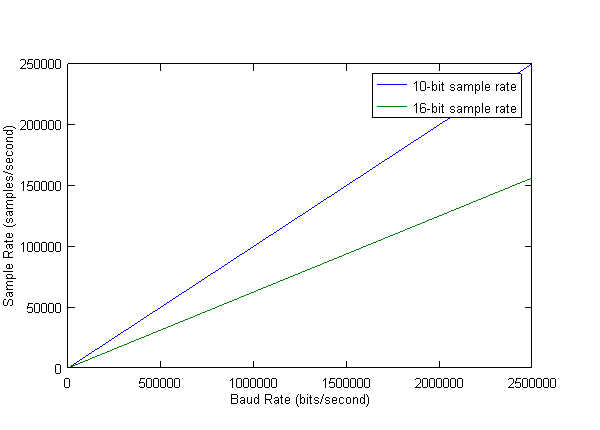
\includegraphics[width=3in]{baud_rate.png}
\end{center}
\label{fig:baud rates and sample}
\end{figure}
\subsection{Cost and Implementation}

Table \ref{tab:datap costs} summarizes the costs involved in implementing the 
datapath control subsystem. The circuit board printing costs are an estimate, 
and assume that low cost is prioritized over production speed. Also, the board
costs are expected to be combined with the power subsystem itself. All costs 
are for the recommended vendors and at low quantities.

\begin{table}[hbp!]
\caption{Pricing information for subsystem components\cite{web:batchpcb}\cite{web:jameco_atmel}\cite{web:jameco_inv}\cite{sparkfun}.}
\small
\begin{center}
\begin{tabular}{l | c c r}
	Item & Quantity & Unit Cost & Total Cost \\ \hline
	Printed Circuit Board & 1 & \$50 & \$50 \\
	ATMega8515(L) (PLCC) & 2 & \$4.58 & \$9.16 \\
	74AC04 & 1 & \$0.056 & \$0.056\\
	74AC245  & 10 & \$0.089 & \$0.89\\
	Headers & 2 & \$2.95 &  \$5.90
\end{tabular}
\end{center}
\label{tab:datap costs}
\end{table}

The PCB fabrication lead time is variable, lasting from either days at a high
 cost per board or weeks at a low cost per board. For hobbyists, it is 
preferable to wait the extra time. Once the board has been printed, the rest of
 the components can be assembled within a few hours, given experience with a 
soldering iron and a steady hand. This design may also be machine-assembled if 
mass-production is desired. Hobbyists may also opt to attempt to etch their own
 circuit boards; but this is not recommended because the net routing is 
difficult to complete satisfactorily. Pin headers were chosen for linking the datapath control to the input modules for their flexibility in accepting connections, but slot connecters could be substituted.

\subsection{Fault Analysis}
Both the MCU and SCU require each other to boot the acquisition unit. A fault 
in the SPI bus interface between them would hang the system or place it into an
unknown state. The data output of the acquisiton unit is invalid while a control
switch is being made. The MCU is sensitive to bad data; the user, if operating
the device, can activate both input modules at once. The behavior in this case
is undefined. However, the included PC software disallows this state.

The SCU and the Wireless Link must have their USART settings set identically for any communication to take place. In order to send commands to the Wireless Link
stack, the flow of data must be halted. During this time, no data is sent to the
Host PC.  

\subsection{Recommendations for Further Study and Conclusions}
Several enchancements can be made to the design of the datapath controllers.
An in-system programming interface may be added to the overall design to allow
for updates to the microcontroller's firmware. These updates could allow for 
changes to control protocols or the addition of new data protocols. Such an 
interface would be relatively inexpensive to add, costing mainly space on the 
controller board.

The prototype implemented utilized a mix of 5V-supply and 3.3V-supply ICs. The 
power supply subsystem can be simplified if all of the components used a single
supply voltage (likely 3.3V). This change is nearly transparent and thus is included in the parts listing as the recommended design.

Performance may be enchanced by utilizing more powerful microcontrollers with
higher clock speeds for the SCU in particular and possibly the MCU. Increasing 
the capability of the SCU relaxes the bottleneck in the serialization, allowing for greater performance. The on-board wireless protocol stack processor may be 
utilized for such a function, but such a change requires 

The design at present makes a useful low-performance device for hobbyists but 
does not have the necessary speed for fast digital logic acquisition and 
analysis. 
